\chapter{Multipoles of the Bispectrum}
\label{chapter:multipoles}

Above the equality scale the galaxy bispectrum will be  a key probe for measuring primordial non-Gaussianity which can help differentiate between different inflationary models and other theories of the early universe. On these scales a variety of relativistic effects come into play once the galaxy number-count fluctuation is projected onto our past lightcone. By decomposing the Fourier-space bispectrum into invariant multipoles about the observer's line of sight we examine in detail how the relativistic effects contribute to these. We show how to perform this decomposition analytically, which is significantly faster for subsequent computations.  While all multipoles receive a contribution from the relativistic part, odd multipoles arising from the imaginary part of the bispectrum have no Newtonian contribution, making the odd multipoles a smoking gun for a relativistic signature in the bispectrum for single tracers.  The dipole and the octopole are significant on equality scales and above where the Newtonian approximation breaks down. This breakdown is further signified by the fact that the even multipoles receive a significant correction on very large scales.

\subsection*{Introduction}
The bispectrum will play a key role in future galaxy surveys as an  important probe of large-scale structure and for measuring primordial 
non-Gaussianity and galaxy bias~\cite{Jeong:2009vd,Baldauf:2010vn,Celoria:2018euj}. It can help discriminate between different inflationary models and other theories of the early universe, and contains information that is complementary and additional to what is contained in the power spectrum. 
On super-equality scales, a variety of relativistic effects come into play once the galaxy number-count fluctuation is projected onto the past light cone. In the density contrast up to second order, relativistic effects arise from observing on the past lightcone, and they include all redshift, volume and lensing distortions and couplings between these. In Poisson gauge, these effects can be attributed to velocities (Doppler), gravitational potentials (Sachs-Wolfe, integrated SW, time delay) and lensing magnification and shear. In addition, there are corrections arising from a GR definition of galaxy bias~\cite{Bertacca:2014wga}. These effects generate corrections to the Newtonian approximation at order $\mathcal{O}(\cH/k)$ and higher. Non-Gaussianity generated by these relativistic projection effects could closely mimic the signature of \(\fnl\) on large scales which gives a correction in the halo bias $\mathcal{O}((\cH/k)^2)$, indicating the importance of precisely including all $\mathcal{O}(\cH/k)$ and higher effects in theoretical modelling. So far, a variety of relativistic effects in the galaxy Fourier bispectrum has been taken into account, see 
\cite{Umeh:2016nuh,Jolicoeur:2017nyt,Jolicoeur:2017eyi,Jolicoeur:2018blf,Clarkson:2018dwn,Maartens:2019yhx} under the assumption of the plane parallel approximation, and neglecting integrated effects. Other groups are working on this from different angles and approaches, for example by a spherical-Fourier formalism~\cite{Bertacca:2017dzm}, and calculating the angular galaxy bispectrum~\cite{DiDio:2016gpd,DiDio:2018unb}. Crucially, we have shown that the relativistic part should be detectable in a survey like Euclid without resorting to the multi-tracer technique, which is needed for the power spectrum~\cite{Maartens:2019yhx} . 

Once an observable like the galaxy number-count fluctuation is projected onto the past lightcone the orientation of the triangle in the Fourier space bispectrum becomes important. 
Analogously to how the Legendre multipole expansion is used for power spectrum analysis, one can expand the galaxy bispectrum in spherical harmonics, thus isolating the different invariant multipoles with respect to the observer's line of sight $\bm n$. We use the full spherical harmonics for the bispectrum rather than the Legendre polynomial expansion usually adopted for the power spectrum because of the azimuthal degrees of freedom associated with the orientation of the triangle with respect to the line of sight direction vector in Fourier space. In the power spectrum limit, there is only one angular degree of freedom after ensemble averaging. For the bispectrum, we have one angular and one azimuthal degree of freedom which when expanded in spherical harmonics leads to $(2\ell + 1)$ independent harmonics for each multipole value $\ell$. 

This has been done for the Newtonian bispectrum, which generates non-zero multipoles only for even 
\(\ell\) (up to \(\ell = 8\)) due to redshift-space distortions~\cite{Scoccimarro:1999ed,Nan:2017oaq}. Contrary to the Newtonian bispectrum, the relativistic galaxy bispectrum generates non-zero multipoles for both even and odd \(\ell\) up to \(\ell = 8\) and \(m = 6\) where the odd multipoles are induced by the general relativistic effects only. This means that these multipoles are a crucial signature of relativistic projection effects. We provide, for the first time, a multipole decomposition of the Fourier space galaxy bispectrum with relativistic effects included. Additionally we show that the coefficients of this expansion can be worked out analytically. We provide an exact analytic formula for this multipole expansion of the galaxy bispectrum. Previously, we examined for the first time the dipole of the galaxy bispectrum in detail, showing that its amplitude can be more than 10\% of that of the monopole even at equality scales~\cite{Clarkson:2018dwn}. 
In order to eliminate possible biases when analysing large scale structure data, it is important to include the relativistic effects. In addition to this, a variety of the effects that appear in the bispectrum are relativistic effects that have not been measured elsewhere and hence are interesting to study. By analysing the non-zero multipoles of the galaxy bispectrum both for a Euclid-like galaxy survey, and for an SKA-like HI intensity mapping survey, we show the behaviour of the higher multipoles and their corrections to the Newtonian bispectrum. In follow-up work, we are investigating possibilities of detecting the higher multipoles of the bispectrum. See for example~\cite{Maartens:2019yhx} for detection prospects of the leading order relativistic effects; the dipole is expected to have the strongest GR signature. 

The paper is organised as follows. We introduce the relativistic Fourier space bispectrum in section~\ref{sec:relbisp}, and present the multipole expansion of the relativistic bispectrum in section~\ref{sec:extrmulti}. An analysis of the multipoles can be found in section~\ref{sec:anal}. Finally, we summarise our conclusions in section~\ref{sec:concl}.

\subsection*{The relativistic bispectrum}\label{sec:relbisp}

In Fourier space, the observed galaxy bispectrum \(B_g\) at a fixed redshift \(z\) is given by~\cite{Jolicoeur:2017nyt,Jolicoeur:2017eyi}
\begin{equation}
	\langle \Delta_g(z,\ka) \Delta_g(z,\kb) \Delta_g(z,\kc) \rangle = (2\pi)^3 B_g(z,\ka,\kb,\kc) \delta^D(\ka+\kb+\kc),
\end{equation}
where \(\Delta_g(z, \ka)\) is the number count contrast at redshift \(z\) (see~\cite{Jolicoeur:2017nyt} for the full expression). Here we work in the Poisson gauge; note that \(\Delta_g = \delta_g + \text{RSD}+\text{GR}\) projection effects, where the RSD term is the Kaiser RSD up to second order, which is part of the Newtonian approximation. Since redshift is fixed, in what follows we drop redshift dependence for brevity. Furthermore, since the observed direction \(\n\) is fixed in what follows, the plane-parallel approximation is necessarily assumed. Then, at tree level, and for Gaussian initial conditions, the following combinations of terms contribute, 
\begin{equation}
\langle \Delta_g(\ka)\Delta_g(\kb)\Delta_g(\kc) \rangle = \frac{1}{2} \langle \Delta_g^{(1)}(\ka)\Delta_g^{(1)}(\kb)\Delta_g^{(2)}(\kc)\rangle \text{ + 2 cyclic permutations.}
\end{equation}
Using Wick's theorem, this gives an expression for the galaxy bispectrum ~\cite{Jolicoeur:2017nyt}
\begin{equation}
B_g(\ka, \kb,\kc)= \ko^{(1)}(\ka) \ko^{(1)}(\kb) \ko^{(2)}(\ka,\kb,\kc)P(\ka) P(\kb)\text{ + 2 cyclic permutations},
\end{equation}
where \(P\) is the power spectrum of \(\delta_\mathrm{T}^{(1)}\), the first order dark matter density contrast in the total-matter gauge, which corresponds to an Eulerian frame. The first order kernel can be split into a Newtonian and a relativistic part as~\cite{Jeong_2012}
\begin{equation}
\ko^{(1)} = \ko^{(1)}_\mathrm{N} + \ko^{(1)}_\mathrm{GR}, \qquad \ko^{(1)}_\mathrm{N}= b_1 + f \mu^2, \qquad \ko^{(1)}_\mathrm{GR} = \i \mu \frac{\gamma_1}{k} + \frac{\gamma_2}{k^2}, 
\end{equation}
with \(\mu = \hat\k \cdot \n \) (\(\hat\k = \k/k\)), \(b_1\) is the first-order Eulerian galaxy bias coefficient, \(f\) is the linear growth rate of matter perturbations, and redshift-dependent coefficients \(\gamma_i\) are~\cite{Jeong_2012},
\begin{align}\label{eq:gamma1def}
\frac{\gamma_1}{\cH} &= f \left[ b_e - 2 \Q - \frac{2(1-\Q)}{\chi \cH} - \frac{\cH'}{\cH^2}\right], \\
\frac{\gamma_2}{\cH^2} &= f(3-b_e) + \frac{3}{2} \Omega_m \left[ 2+ b_e - f - 4\Q - \frac{2(1-\Q)}{\chi\cH} - \frac{\cH'}{\cH^2} \right].\label{eq:gamma2def}
\end{align}
In equations~\eqref{eq:gamma1def}~and~\eqref{eq:gamma2def}, \(\cH\) is the conformal Hubble rate \((\ln a)'\), where a prime denotes a derivative with respect to conformal time; \(b_e\) and \(\Q\) are the galaxy evolution and magnification biases respectively, \(\chi\) is the line-of-sight comoving distance and \(\Omega_m = \Omega_{m0} (1+z) H_0^2/\cH^2\) is the matter density parameter. At first order, the gauge-independent GR definition of galaxy bias is made in the common comoving frame of galaxies and matter, 
\begin{equation}\label{eq:comovinggalaxybiasdef}
	\delta_{g\mathrm{C}}^{(1)} = b_1 \delta_\mathrm{C}^{(1)} =  b_1 \delta_\mathrm{T}^{(1)}\,,
\end{equation}
where subscript C is for the comoving gauge and T is for total matter gauge, which is a gauge corresponding to standard Newtonian perturbation theory. The bias relation in Poisson gauge is then obtained by transforming~\eqref{eq:comovinggalaxybiasdef} to Poisson gauge~\cite{Bertacca:2014wga,Jolicoeur:2017eyi}:
\begin{equation}\label{eq:deltareln}
	\delta_g^{(1)} = \delta_{g\mathrm{C}}^{(1)} + (3 - b_e)\cH v^{(1)} = b_1 \delta_\mathrm{T}^{(1)} + (3-b_e)\cH v^{(1)},
\end{equation}
where \(v^{(1)}\) is the velocity potential. Since \(v^{(1)} =f \cH \delta_T^{(1)}/k^2\), the last term on the right of equation~\eqref{eq:deltareln} leads to the \(f(3-b_e)\) term in \(\gamma_2/\cH^2\), equation~\eqref{eq:gamma2def}.


Similarly to the first order kernel, the second order kernel can be split into a Newtonian and a relativistic part. The second order part of the Newtonian kernel is well studied and is given as~\cite{Bernardeau_2002,Karagiannis_2018,Scoccimarro:1999ed,Verde:1998zr}
\begin{align}\label{newt2o}
	\ko_\mathrm{N}^{(2)}(\ka, \kb, \kc) &= b_1 F_2(\ka,\kb) + b_2 + f \mu_3^2 G_2(\ka,\kb) + f Z_2(\ka,\kb) + b_{s^2} S_2(\ka,\kb),
\end{align}
where \(\mu_i = \hat\k_i \cdot \n \), \( b_2\) is the second-order Eulerian bias parameter, and \(b_{s^2} \) is the tidal bias. \(F_2\) and \(G_2\) are the Fourier-space Eulerian kernels for second-order density contrast and velocity respectively~\cite{Jolicoeur:2017nyt,Villa:2015ppa}; 
\begin{align}
F_2(\ka,\kb) &= 1 + \frac{F}{D^2} + \left(\hat{\k}_1 \cdot \hat{\k}_2 \right)\left( \frac{k_1}{k_2} + \frac{k_2}{k_1}\right) + \left( 1-\frac{F}{D^2}\right) \left(\hat{\k}_1 \cdot \hat{\k}_2 \right)^2,\nonumber \\
G_2(\ka,\kb) &= \frac{F'}{D D'} + \left(\hat{\k}_1 \cdot \hat{\k}_2\right)\left(\frac{k_1}{k_2} + \frac{k_2}{k_1} \right) + \left( 2 - \frac{F'}{D D'} \right) \left(\hat{\k}_1 \cdot \hat{\k}_2\right)^2,
\end{align}
where \(F\) is a second-order growth factor, which is given by the growing mode solution of,
\begin{equation}
F'' + \cH F' - \frac{3}{2}\frac{H_0^2 \Omega_{m0}}{a} F = \frac{3}{2}\frac{H_0^2 \Omega_{m0}}{a} D^2.
\end{equation}
 In an Einstein-de Sitter background, \(F= 3 D^2 / 7\), which is a very good approximation for \(\Lambda\)CDM which we use here. The second-order RSD part of the Newtonian kernel is comprised of \(G_2\) above and the kernel \(Z_2\)~\cite{Verde:1998zr,Scoccimarro:1999ed},
\begin{equation}
	Z_2(\ka,\kb) = f \frac{\mu_1 \mu_2}{k_1 k_2}\left( \mu_1 k_1 + \mu_2 k_2 \right)^2 + \frac{b_1 }{k_1 k_2} \left[ \left( \mu_1^2 + \mu_2^2 \right)k_1 k_2 + \mu_1 \mu_2 \left( k_1^2 + k_2^2 \right) \right]\,.
\end{equation}

 Finally, \(S_2(\ka,\kb)\) is the kernel for the tidal bias,
\begin{equation}
	S_2(\ka,\kb) = (\hat{\k}_1 \cdot \hat{\k}_2)^2 - \frac{1}{3}\,.
\end{equation}
The Newtonian bias model is 
\begin{equation}\label{eq:newtbiasmodel}
	\delta_{g\mathrm{T}}^{(2)} = b_1 \delta_\mathrm{T}^{(2)} + b_2 \left[\delta_\mathrm{T}^{(1)}\right]^2 + b_{s^2} s^2\,,
\end{equation}
where \( s^2 = s_{ij}s^{ij}\), and \( s_{ij} = \Phi_{,ij} - \delta_{ij}\nabla^2 \Phi /3\) . 

The relativistic part of the second order kernel was first derived in~\cite{Umeh:2016nuh} in the simplest case and extended in~\cite{Jolicoeur:2017nyt,Jolicoeur:2017eyi,Jolicoeur:2018blf}. Neglecting sub-dominant vector and tensor contributions, we have 
\begin{align}\label{eq:soGRkernel}
\ko_\mathrm{GR}^{(2)}(\ka,\kb,\kc) &= \frac{1}{k_1^2 k_2^2} \left\{ \vphantom{\frac{k_1^2 k_2^2}{k_3}} \beta_1 + E_2(\ka,\kb,\kc) \beta_2 
+\i (\mu_1k_1+\mu_2k_2)\beta_3
+ \i \mu_3 k_3\left[ \beta_{4} + E_2(\ka, \kb, \kc)\beta_{5}\right] \right. \nonumber \\
&\left. +\frac{k_1^2 k_2^2}{k_3^2} \left[ F_2(\ka,\kb) \beta_{6} + G_2(\ka,\kb) \beta_{7} \right] + \left( \mu_1 k_1 \mu_2 k_2 \right)\beta_{8} + \mu_3^2 k_3^2 \left(\beta_{9} + E_2(\ka,\kb,\kc) \beta_{10} \right) \right. \nonumber \\
&\left. + \left(\ka \cdot \kb \right)\beta_{11} + \left( k_1^2 + k_2^2 \right) \beta_{12} + \left( \mu_1^2 k_1^2 + \mu_2^2 k_2^2 \right) \beta_{13} \right. \nonumber \\
&\left. + \i \left[\vphantom{\frac{k_1^2 k_2^2}{k_3}} \left( \mu_1 k_1^3 + \mu_2 k_2^3 \right)\beta_{14} + \left( \mu_1 k_1 + \mu_2 k_2 \right) \left(\ka\cdot\kb \right) \beta_{15} + k_1 k_2 \left(\mu_1 k_2 + \mu_2 k_1 \right) \beta_{16} \right. \right. \nonumber \\
&\left. \left. + \left( \mu_1^3 k_1^3 + \mu_2^3 k_2^3 \right)\beta_{17} + \mu_1 \mu_2 k_1 k_2 \left( \mu_1 k_1 + \mu_2 k_2 \right) \beta_{18} + \mu_3 \frac{k_1^2 k_2^2}{k_3} G_2(\ka,\kb) \beta_{19} \right] \right\}.
\end{align}
We have collected terms according to the overall powers of $k$ involved.
The \(\beta_i\) here are redshift- and bias-dependent coefficients, given in full in appendix  REF BETA APPENDIX, which updates  expressions in previous papers.
We have defined the kernel \(E_2\) which scales as \(k^0\) (like \(F_2\), \(G_2\), and \(Z_2\) do), 
\begin{equation}
E_2(\ka,\kb,\kc) = \frac{k_1^2 k_2^2}{k_3^4} \left[ 3 + 2 \left( \hat{\k}_1 \cdot\hat{\k}_2 \right) \left( \frac{k_1}{k_2} + \frac{k_2}{k_1} \right) + \left( \hat{\k}_1 \cdot \hat{\k}_2 \right)^2 \right],
\end{equation}
which incorporates some of the relativistic dynamical corrections to the intrinsic second-order terms.

At second order, the GR bias model, which corrects the Newtonian bias model~\eqref{eq:newtbiasmodel} is given by~\cite{Umeh:2019qyd},
\begin{equation}
	\delta_{g\mathrm{T}}^{(2)} = b_1 \delta_\mathrm{T}^{(2)} + b_2 \left[ \delta_\mathrm{T}^{(1)} \right]^2 + b_{s^2} s^2 + \delta_{\mathrm{C,GR}}^{(2)}\,,
\end{equation}
where the last term maintains gauge invariance on ultra-large scales, and is given by (using \( \delta_\mathrm{C}^{(1)} =  \delta_\mathrm{T}^{(1)}\) )
\begin{equation}\label{eq:grcorrdelta}
	\delta_{\mathrm{C,GR}}^{(2)} = 2 \cH^2 (3 \Omega_m + 2 f) \left[ \delta_\mathrm{T}^{(1)} \nabla^{-2} \delta_\mathrm{T}^{(1)} - \frac{1}{4} \partial_i \nabla^{-2} \delta_\mathrm{T}^{(1)} \partial^i \nabla^{-2} \delta_\mathrm{T}^{(1)} \right]\,.
\end{equation}
The GR correction~\eqref{eq:grcorrdelta} to the Newtonian bias model is contained in the GR kernel~\eqref{eq:soGRkernel}. Then, we also need to transform \(\delta_{g\mathrm{T}}^{(2)}\) to the Poisson	 gauge \( \delta_g^{(2)} \), the expression for this is given in~\cite{Jolicoeur:2017nyt}, 
\begin{align}
\delta_{g}^{(2)}  &= \delta_{g{\mathrm{T}} }^{(2)} + (3-b_e) \cH v^{(2)} +\Big[ (b_e-3) \cH' + b_e' \cH + (b_e-3)^2 \cH^2 \Big]  \big[v^{(1)}\big]^2 + (b_e-3)\cH   v^{(1)}  v^{(1)\prime} \nonumber\\
& +2(3-b_e)\cH  v^{(1)} \delta_{g{\mathrm{T}}}^{(1)}  - 2  v^{(1)} \delta_{g{\mathrm{T}}}^{(1)\prime} + 3 \left( b_e-3\right) \cH v^{(1)}\Phi^{(1)} \,.\label{dgpt}
\end{align}
All of the terms after $\delta_{g\mathrm{T}}^{(2)}$ on the right of equation~\eqref{dgpt} scale as $(\cH/k)^n \left[ \delta^{(1)}_\mathrm{T} \right]^2$, where $n = 2,4$. Therefore they are omitted in the Newtonian approximation. These GR correction terms maintain gauge-independence on ultra-large scales, and they are included in the GR kernel~\eqref{eq:soGRkernel}.


\subsection*{Extracting the multipoles}\label{sec:extrmulti}

Our goal is to extract the spherical harmonic multipoles of $B_g$ with respect to the observer's line of sight. That is, for a fixed line of sight and triangle shape, the rotation of the plane of the triangle about $\n$ generates invariant moments, the sum of which add up to the full bispectrum. 
 This means that  
\begin{equation}
B_g =\sum_{\ell m} B_{\ell m}Y_{\ell m}(\n)\,,
\end{equation}
where we follow~\cite{Scoccimarro:1999ed,Nan:2017oaq} in our choice of decomposition of the bispectrum (an alternative basis can be found in~\cite{Sugiyama_2018}).
To define the $B_{\ell m}$ we need to define an orientation for the $Y_{\ell m}$ to give the polar and azimuthal angles over which to integrate. We choose a coordinate basis for the vectors that span the triangle as follows: 
\begin{eqnarray}
	&&\k_1 = (0,0,k_1)\, \\
	&&\k_2 = (0, k_2 \sin\theta, k_2 \cos\theta)\,, \\
	&&\k_3 = (0, - k_2 \sin\theta, - k_1 - k_2\cos\theta )\,,\\
	&&\bm{n} = (\sin\theta_1 \cos\varphi, \sin\theta_1 \sin\varphi,\cos\theta_1)\,.
\end{eqnarray}
That is, we fix $\k_1$ along the $z$-axis, and require the other triangle vectors to lie in the $y$-$z$ plane, see figure~\ref{fig:geometry_overview} for a sketch of the relevant vectors. Then we define {\(\mu_1=\cos\theta_1\)} and use $\varphi$, which is the azimuthal angle giving the orientation of the triangle relative to $\n$. \(\theta_{12} = \theta\) is the angle between vectors \(\k_1\) and \(\k_2\), and we define $\mu=\cos\theta=\hat{\k}_1\cdot\hat{\k}_2$.
\begin{figure}[ht]
	\centering
	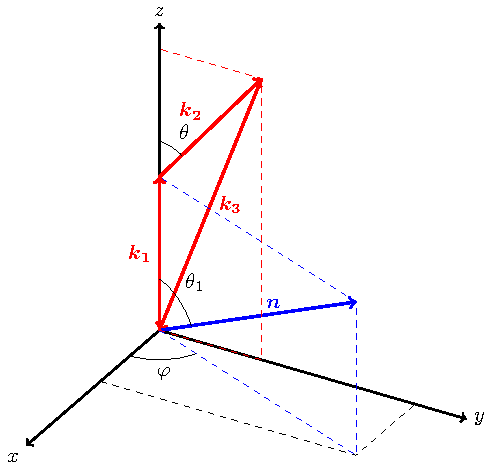
\includegraphics[width=0.6
	\linewidth]{fig/fig.pdf}
	\caption{Overview of the relevant vectors and angles for the Fourier-space bispectrum. \label{fig:geometry_overview} }
\end{figure}

The bispectrum can then be expressed in terms of five variables, \(\varphi\), \(\mu_1\), \(\theta\), \(k_1\) and \(k_2\), by using
\begin{align}
	\mu_2 &= \sqrt{1-\mu_1^2} \sin\theta \sin\varphi + \mu_1\cos\theta\,,  \\
	\mu_3 &= -\frac{k_1}{k_3}\mu_1 - \frac{k_2}{k_3}\mu_2.
\end{align}
Then 
\begin{equation}\label{eq:bgexpv1}
	B_g(\theta, k_1, k_2, \mu_1, \varphi) = \sum_{\ell m} B_{\ell m}(\theta, k_1, k_2) Y_{\ell m} (\mu_1, \varphi)\,,
\end{equation}
where we use standard orthonormal spherical harmonics,
\begin{equation}
	Y_{\ell m}(\mu_1,\varphi) = \sqrt{\frac{2\ell+1}{4 \pi}} \sqrt{\frac{(\ell-m)!}{(\ell+m)!}} P_\ell^m(\mu_1) e^{{\i} m \varphi},
\end{equation}
where the \(P_\ell ^m\) are the associated Legendre polynomials, 
\begin{equation}
	P_\ell ^m(\mu_1) = \frac{(-1)^m}{2^\ell \,\ell !} (1-\mu_1^2)^{m/2} \frac{{\diff}^{\ell +m}}{{\diff}\mu_1^{\ell +m}}(\mu_1^2 - 1)^\ell . 
\end{equation}
At this stage we can extract the multipoles numerically once a bias model and cosmological parameters are given. It is actually significantly quicker to perform this extraction algebraically however, as we now explain. 

The bispectrum in general can be considered as a function of
$k_1,k_2,k_3,\mu,\mu_1, \mu_2, \mu_3$ and $\varphi$. An alternative to the expansion~\eqref{eq:bgexpv1} is 
\begin{equation}\label{eq:bg_absum_reln}
B_g (\mu,k_1,k_2;\mu_1,\mu_2)= \sum_{a=0}^6\sum_{b=0}^6 \mathcal{B}_{ab}(\mu, k_1, k_2)  (\i\mu_1)^a(\i\mu_2)^b\,,
\end{equation}
where we used $\mu_2$ instead of $\varphi$ and $a,b=0\ldots6$, which is the maximum power of $\mu_1,\,\mu_2$ that can arise. This factors out all the angular dependence from the functions $\mathcal{B}_{ab}(\mu,k_1,k_2)$, where $\mu=\cos\theta$, which just depend on the triangle shape (and the cosmology). Note that by explicitly including factors of $\i$ in the sum, we have only real coefficients $\mathcal{B}_{ab}$. 
Schematically we can visualise $\mathcal{B}_{ab}$ in matrix form, split into Newtonian and relativistic contributions as (a bullet denotes a non-zero entry, open circles denote zero entries, and dots are non-existent entries; here that means $a+b > 8$ as higher powers don't occur):
\begin{equation} \label{eq:bab_newtrelmatrix}
\mathcal{B}_{ab}\sim  \underbrace{ 	
\left( 
\begin {array}{ccccccc}  
\bullet& \circ &\bullet& \circ &\bullet& \circ & \circ \\  
\circ  &\bullet& \circ  &\bullet& \circ &\bullet& \circ \\  
\bullet& \circ &\bullet& \circ &\bullet&  \circ&\bullet\\  
\circ  &\bullet& \circ &\bullet& \circ &\bullet& \cdot \\  
\bullet& \circ &\bullet& \circ &\bullet& \cdot &  \cdot\\  
\circ  &\bullet& \circ &\bullet&  \cdot & \cdot & \cdot \\  
\circ  & \circ &\bullet& \cdot & \cdot & \cdot &  \cdot 
\end {array} 
\right)
%\begin{blockarray}{rccccccc}
%a=&~0~&~1~&~2~&~3~&~4~&~5~&~6~\\
%\begin{block}{r(ccccccc)}
%b=0~~&\bullet& \circ &\bullet& \circ &\bullet& \circ & \circ \\  
%1~~&\circ  &\bullet& \circ  &\bullet& \circ &\bullet& \circ \\  
%2~~&\bullet& \circ &\bullet& \circ &\bullet&  \circ&\bullet\\  
%3~~&\circ  &\bullet& \circ &\bullet& \circ &\bullet& \cdot \\  
%4~~&\bullet& \circ &\bullet& \circ &\bullet& \cdot &  \cdot\\  
%5~~&\circ  &\bullet& \circ &\bullet&  \cdot & \cdot & \cdot \\  
%6~~&\circ  & \circ &\bullet& \cdot & \cdot & \cdot &  \cdot \\
%\end{block}
%\end{blockarray}
}_\text{Newtonian}
+
\underbrace{\left( \begin {array}{ccccccc}   \bullet & \bullet & \bullet & \bullet & \bullet & \bullet & \bullet \\   \bullet & \bullet & \bullet & \bullet & \bullet & \bullet & \bullet \\   \bullet & \bullet & \bullet & \bullet & \bullet & \bullet & \circ  \\   \bullet & \bullet & \bullet & \bullet & \bullet & \circ  & \cdot  \\   \bullet & \bullet & \bullet & \bullet & \circ  & \cdot  & \cdot  \\   \bullet &
 \bullet & \bullet &\circ   & \cdot  & \cdot  & \cdot  \\   \bullet & \bullet & \circ  &\cdot   &  \cdot &  \cdot 
& \cdot  \end {array} \right)}_\text{Relativistic}\,.
\end{equation}
(Note that the matrix row and column labelling start at $a,b=0,0$ for the top left element.) 
Thus, the Newtonian contributions always have $a+b=$\,even\,$\leq8$, contributing only to the real part of $B_g$, while there are relativistic contributions present for all $a+b\leq7$. When $a+b$ is odd, this implies an imaginary component to the full bispectrum.  

In terms of the powers of $\cH/k$ involved, we can visualise the maximum powers that appear in matrix form as follows:
\begin{equation}  \label{eq:maxpowerkmatrix}
\mathcal{B}_{ab}\sim \left( \begin {array}{ccccccc} {k}^{-8}&{k}^{-7}&{k}^{-6}&{k}^{-5}&{k
}^{-4}&{k}^{-3}&{k}^{-2}\\  
{k}^{-7}&{k}^{-6}&{k}^{-5
}&{k}^{-4}&{k}^{-3}&{k}^{-2}&{k}^{-1}\\  
{k}^{-6}&{k}
^{-5}&{k}^{-4}&{k}^{-3}&{k}^{-2}&{k}^{-1}&k^0\\  
{k}^{-
5}&{k}^{-4}&{k}^{-3}&{k}^{-2}&{k}^{-1}&k^0 & \cdot\\  
{k}^{-4
}&{k}^{-3}&{k}^{-2}&{k}^{-1}&k^0 &\cdot &\cdot \\  
{k}^{-3}&{k}^{-
2}&{k}^{-1}&k^0 & \cdot&\cdot &\cdot \\  
{k}^{-2}&{k}^{-1}&k^0 &\cdot & \cdot&\cdot & \cdot
\end {array} \right) \,.
\end{equation}

As in the matrix~\eqref{eq:bab_newtrelmatrix}, the matrix row and column labelling in~\eqref{eq:maxpowerkmatrix} starts at $(a,b) = (0,0)$. We see that higher powers $n$ of $(\cH/k)^n$ appear for lower $a+b$. Newtonian contributions are all $({\cal H}/k)^0$. Each element has only odd powers of $\cH/k$ if $a+b$ is odd, and similarly only even powers if $a+b$ is even.

The advantage of writing the bispectrum in this form is that we can derive analytic formulas for the multipoles. We need to find
\begin{align}
B_{\ell m} &= \int{\diff}\Omega \,\,B_g Y^*_{\ell m} \nonumber \\
&= \sum_{a,b} \mathcal{B}_{ab} X_{\ell m}^{ab} \label{eq:xabexp} \,,
\end{align}
where 
\begin{equation} X_{\ell m}^{ab} = \int_0^{2\pi} \diff\varphi\, \int_{-1}^1 \diff\mu_1\, (\i \mu_1)^a (\i \mu_2)^b \,Y_{\ell m}^*(\mu_1,\varphi).
\end{equation}
To do this we use the identity, derived in appendix REF APPENDIX WITH SUM DERIVATION, for $m \geq 0$,
\begin{align}\label{eq:sumformula} X_{\ell m}^{ab} &= 2^{\ell+m-1}\i^{a+b+m}\sqrt{\frac{\pi(2\ell+1)(\ell-m)!}{(\ell+m)!}}\nonumber\\
&\times
\sum_{p=m}^{\frac{1}{2}(b+m)}\sum_{q=m}^{\ell}
\frac{[1+(-1)^{a+b+q}]\,b!\,\cos^{b+m-2p}\theta\sin^{2p-m}\theta}{4^p(b+m-2p)!(\ell-q)!(p-m)!(q-m)!}
%\frac{[\frac{1}{2}(q+\ell-1)]!}{[\frac{1}{2}(q-\ell-1)]!}
%\frac{[\frac{1}{2}(a+b +q-p-1)]!}{[\frac{1}{2}(a+b+q+1)]!}
\frac{\Gamma[\frac{1}{2}(q+\ell+1)]}{\Gamma[\frac{1}{2}(q-\ell+1)]}
\frac{\Gamma[\frac{1}{2}(a+b +q-2p+1)]}{\Gamma[\frac{1}{2}(a+b+q+3)]}
\end{align}
for $m\leq b$ and zero otherwise. For $m < 0$, the result follows a similar pattern, using the simple relation \(X_{\ell -m}^{ab} = (-1)^{a+b+m} X_{\ell m}^{ax`'b*}\), see appendix REF DERIVATION SUM APPENDIX. 

The resulting expressions for $B_{\ell m}$ are rather massive, in part because the cyclic permutations become mixed together, so we do not present them here. We can visualise these in matrix form split into their Newtonian and relativistic contributions:
\begin{equation} \label{eq:blm_newtrelmatrix}
B_{\ell m}=
 \underbrace{\left( \begin {array}{ccccccccc} \bullet& \cdot  &  \cdot& \cdot  &  \cdot& \cdot  &  \cdot& \cdot  &  \cdot
\\  \circ & \circ  &  \cdot& \cdot  &  \cdot& \cdot  &  \cdot& \cdot  &  \cdot \\ \bullet&\bullet&\bullet& \cdot  &  \cdot& \cdot 
& \cdot  &  \cdot& \cdot \\  \circ & \circ  &  \circ& \circ  &  \cdot& \cdot  &  \cdot& \cdot  & \cdot \\ \bullet&\bullet&\bullet
&\bullet&\bullet& \cdot  &  \cdot& \cdot  & \cdot \\ \circ  & \circ  &  \circ& \circ  &  \circ& \circ  &  \cdot& \cdot  & \cdot 
\\ \bullet&\bullet&\bullet&\bullet&\bullet&\bullet&\bullet& \cdot  &  \cdot  \\ \circ  & \circ  &  \circ& \circ  &  \circ&  
\circ & \circ  &  \circ & \cdot \\ \bullet&\bullet&\bullet&\bullet&\bullet&\bullet&\bullet& \circ & \circ \end {array} \right)}_\text{Newtonian}
+
\underbrace{\left( \begin {array}{ccccccccc} \bullet&  \cdot&\cdot  &  \cdot&\cdot  &  \cdot&\cdot  &  \cdot&  \cdot
\\  \bullet&\bullet&  \cdot&\cdot  &  \cdot&\cdot  &  \cdot&\cdot  &  \cdot
\\  \bullet&\bullet&\bullet&  \cdot&\cdot  &  \cdot&\cdot  &  \cdot&  \cdot
\\  \bullet&\bullet&\bullet&\bullet&  \cdot&\cdot  &  \cdot&\cdot  &  \cdot
\\  \bullet&\bullet&\bullet&\bullet&\bullet&  \cdot&\cdot  &  
\cdot & \cdot \\  \bullet&\bullet&\bullet&\bullet&\bullet& \bullet &  \cdot&\cdot  & \cdot \\  \bullet&\bullet&\bullet&\bullet&
\bullet&\bullet&\bullet&  \cdot&  \cdot \\  \bullet&\bullet& \bullet &\bullet&\bullet&\bullet&\bullet& \circ & \cdot \\  \circ  & \circ 
&  \circ&\circ  &  \circ&\circ  &  \circ&\circ  & \circ \end {array} \right)}_\text{Relativistic}\,.
\end{equation}
Again, the matrix indices start at $(0,0$) in the top left, $(\ell,m) = (0,0)$. In the matrix~\eqref{eq:blm_newtrelmatrix}, consistent with previous matrix visualisations, a closed bullet represents a non-zero entry, while an open circle denotes a vanishing entry. The dots denote the non-existent elements of the matrix, here they are matrix elements where \(m > \ell\) and hence do not exist.
So, the Newtonian bispectrum only induces even multipoles up to and including $\ell=8$, while the relativistic part induces even and odd multipoles up to $\ell=7$ with multipoles higher than $\ell = 8$ vanishing exactly. Both the Newtonian and the relativistic part terminate at $m=\pm6$, because $m\leq b\leq6$, as can  be seen from~\eqref{eq:sumformula}. Note that for $m<0$ the pattern is the same.	
In terms of $({\cal H}/k)$ powers, the highest that appear for each $\ell$ is $({\cal H}/k)^{8-\ell}$, while the leading contribution is $({\cal H}/k)^{0~\text{or}~1}$ if the leading contribution is Newtonian or relativistic. These powers are even (odd) if $\ell$ is even (odd), as explained previously along with the visualisation of the powers $\cH/k$ in equation~\eqref{eq:maxpowerkmatrix}.


\subsubsection*{Presentation of the matrix $\mathcal{B}_{ab}$}


\subsection*{Analysis}\label{sec:anal}

Here we present an analysis of the behaviour of the  multipoles. 

\subsubsection*{ Co-linear, squeezed and equilateral limits}

bob

\subsubsection*{Numerical results}

bob

\subsection*{Conclusion}\label{sec:concl}

concl